% Chapter 4

\chapter{Problème 2D et percussion des floes} % 5th chapter title

\label{Chapter4} % For referencing the chapter elsewhere, use \ref{Chapter5} 

%1----------------------------------------------------------------------------------------



Dans cette section, nous étudierons le floe de glace en deux dimention (2D). Nous reprendrons le même chéminement qu'en 1D. En d'autres termes, nous partirons de l'approche approche par réseau de ressort introduite par Balasoiu pour modéliser dans un premier temps le déplacement d'un floe de glace contenant juste trois n\oe{}uds (masses), ensuite nous modéliserons la percussion inélastique sans rebond des n\oe{}uds de floes. 






%2----------------------------------------------------------------------------------------

\section{Dévelopement d'un modèle de déplacement des n\oe{}uds}








Étudions le comportement d'un floe de glace 2D modélisé par un réseau de ressorts (3 ressort, 3 dispositif viseux, et 3 n\oe{}uds) (voir \cref{fig:deplacement2d}).
\begin{figure}[!h]
    \centering
    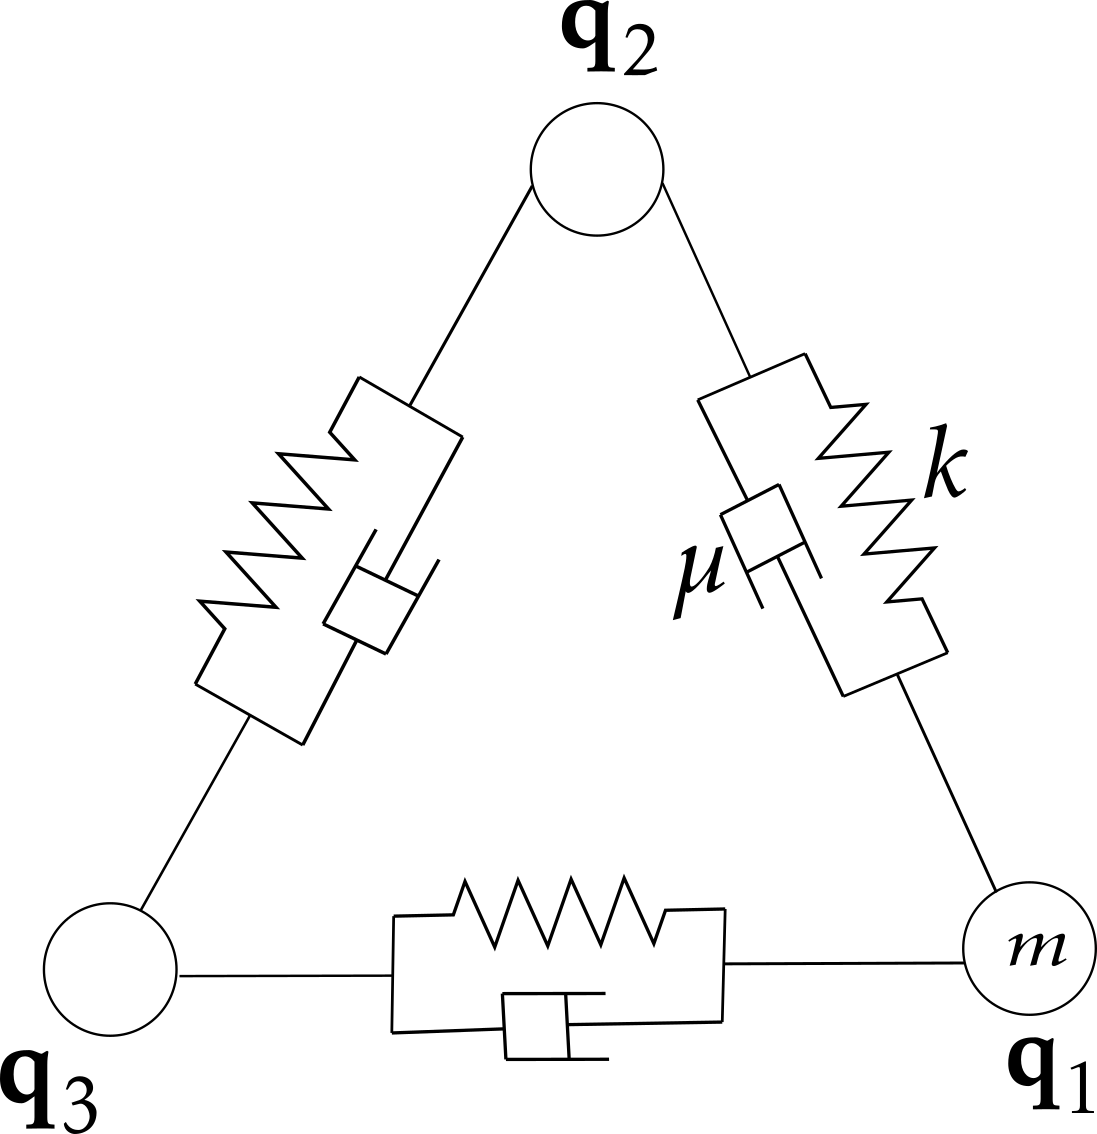
\includegraphics[width=0.3\textwidth]{Deplacement2D-1.png}
    \caption{Floe de glace 2D modélisé par un réseau de ressorts. Le floe est isolé de toutes forces extérieurs. Tous les neouds du réseau ont la même masse $m$, tous les ressorts on la même raideur $k$, et tous les dispositifs visquens ont le même coefficient $\mu$.}
    \label{fig:deplacement2d}
\end{figure}


\noindent Comme nous l'avons présenté aux \cref{eq:F0,eq:e}, le système de la \cref{fig:deplacement2d} est régit par l' équation:
\begin{align} \label{eq:eprime2}
    \forall i \in \mathbb{Z}/3\mathbb{Z}, \quad m \ddot{\bvec{q}}_i = \sum_{j=i+1}^{i+2}C_{ij} \left[  k \left( \Vert \bvec{q}_j - \bvec{q}_i \Vert - L_{ij} \right) \bvec{u}_{ij} - \mu \left\langle \bvec{\dot{q}}_j - \bvec{\dot{q}}_i, \, \bvec{u}_{ij}  \right\rangle  \bvec{u}_{ij}  \right]  , 
\end{align}
où $L_{ij}$ représente la longeur au repos du ressort entre les n\oe{}uds $i$ et $j$, et $C_{ij}$ indique si les n\oe{}uds $i$ et $j$ sont connectés ou non (pour ce modèle 2D simple, $C_{ij} = 1 \, \forall 0 \leq i,j \leq 2$). Le vecteur unitaire $\bvec{u}_{ij}$ vaut:
$$
\bvec{u}_{ij} = \frac{\bvec{q}_j - \bvec{q}_i}{\Vert \bvec{q}_j - \bvec{q}_i \Vert}.
$$


\paragraph{Simulation par un schéma d'Euler explicite.}

On discrétise par un schéma de différence finies avec $N+1$ pas de temps, et pour une temps de simulations $T$:
$$
\forall i \in \mathbb{Z}/3\mathbb{Z}, \, \forall n \in [\![ 0,N ]\!], \quad  t^n = n\Delta t = n\frac{T}{N}, \quad \bvec{q}_i(t^n) \approx \bvec{q}_i^n.
$$
L'\cref{eq:eprime2} devient:
$$
m\frac{\bvec{q}_{i}^{n+1}-2\bvec{q}_{i}^{n}+\bvec{q}_{i}^{n-1}}{\Delta t^2} = \sum_{j=i+1}^{i+2}C_{ij}\left[ k \left( \Vert \bvec{q}_j^n - \bvec{q}_i^n \Vert - L_{ij} \right) \bvec{u}_{ij} - \mu \left\langle \frac{\bvec{q}_{j}^{n}-\bvec{q}_{j}^{n-1}}{\Delta t} - \frac{\bvec{q}_{i}^{n}-\bvec{q}_{i}^{n-1}}{\Delta t}, \, \bvec{u}_{ij} \right\rangle  \bvec{u}_{ij}  \right],
$$
soit encore:
\begin{align} \label{eq:systeme2D}
    \bvec{q}_{i}^{n+1} = 2\bvec{q}_{i}^{n}-\bvec{q}_{i}^{n-1} + \frac{\Delta t^2}{m} \sum_{j=i+1}^{i+2}C_{ij}\left[ k \left( \Vert \bvec{q}_j^n - \bvec{q}_i^n \Vert - L_{ij} \right) \bvec{u}_{ij} - \frac{\mu}{\Delta t} \left\langle \bvec{q}_{j}^{n}-\bvec{q}_{j}^{n-1} - \bvec{q}_{i}^{n}+\bvec{q}_{i}^{n-1}, \, \bvec{u}_{ij} \right\rangle  \bvec{u}_{ij}  \right].
\end{align}
La simulation de ce modèle par un schéma d'Euler explicite à pas constant sur un intervalle de temps faible ($T = 4$) est présentée à la \cref{fig:PlotDeplacement2D1Conv}, ainsi que les positions des 2 n\oe{}uds au début et à la fin de la simulation. La simulation à la \cref{fig:PlotDeplacement2D1NonConv} permet d'observer le problème avec ce schéma ($T = 10$).


\begin{figure}[!h]
    \begin{subfigure}[b]{0.7\textwidth}
        \centering
        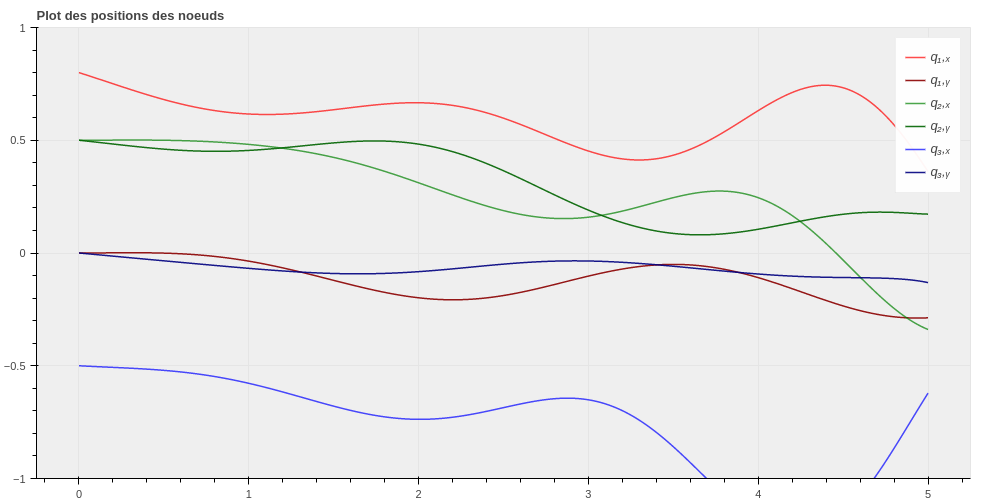
\includegraphics[width=\textwidth]{PlotDeplacement2D-1-Conv.png}
        \caption{Simulation des positions des n\oe{}uds.}
        \label{fig:dep}
    \end{subfigure}
%     \hfill
    \begin{subfigure}[b]{0.7\textwidth}
        \centering
        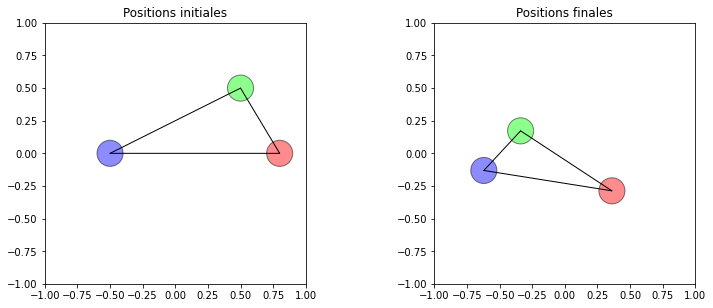
\includegraphics[width=\textwidth]{PositionInitFinales.png}
        \caption{Illustration des positions initiales et finales des neouds.}
        \label{fig:pos}
    \end{subfigure}
    \caption{Simulation du système \ref{eq:systeme2D} par un schéma d'Euler explicite avec $T = 4$ lorsqu'\textbf{un des n\oe{}uds est fixé} (le n\oe{}ud rouge). La couleur rouge repésente le n\oe{}ud $\bvec{q}_1$, le vert le n\oe{}ud $\bvec{q}_2$, le blue le $\bvec{q}_3$. Les paramètres utilisés ici sont les suivants: $m=6.2$, $k=23.3$, $\mu=3$; à l'instant initiale, les trois n\oe{}uds perturbés avec des vitesses d'intensité respectives $v_1=0.3$, $v_2=0.1$, et $v_3=0.1$. Par rapport à l'axe des abcisses, ces vitesses ont sont orintées respectivement de $\theta_1=180^\circ$, $\theta_2=270^\circ$, et $\theta_3=240^\circ$ (voir \texttt{code/simu2D/Deplacement2D-1.ipynb}).}
    \label{fig:PlotDeplacement2D1Conv}
\end{figure}


\begin{figure}[!h]
    \centering
    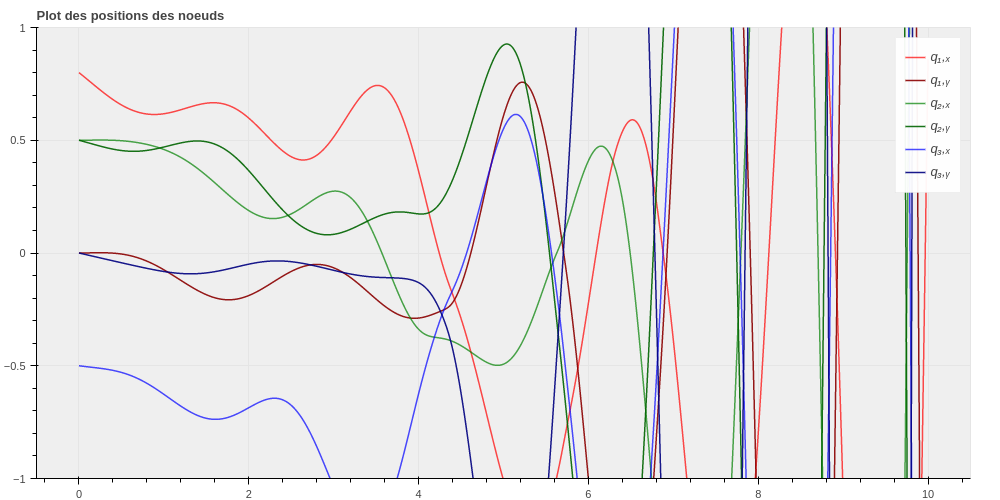
\includegraphics[width=0.7\textwidth]{PlotDeplacement2D-1-NonConv.png}
    \caption{Simulation du système \ref{eq:systeme2D} par un schéma d'Euler explicite avec $T = 10$ lorsqu'\textbf{aucun des n\oe{}uds n'est fixé}. Cette figure utilise les mêmes paramtètres que la \cref{fig:PlotDeplacement2D1Conv}. On observe ici une divergence complète du système (voir \texttt{code/simu2D/Deplacement2D-2.ipynb}).}
    \label{fig:PlotDeplacement2D1NonConv}
\end{figure}

Les \cref{fig:PlotDeplacement2D1Conv,fig:PlotDeplacement2D1NonConv} permettent de constater que le schéma d'Euler explicite (peu importe son pas de temps), n'est pas adapté à ce problème. Nous étudierons donc d'autres alternatives. 

 
\paragraph{Simulation à l'aide des fonctions de la librarie Scipy.} À travers ses fonction telle que \texttt{odeint} et $\verb|solve_ivp|$, \texttt{Scipy} offre une solution robuste et élégante pour simuler les systèmes d'ODE de la forme $Y' = AY$. Avec \texttt{Scipy}, nous résolvons numériquement nos EDO à l'ordre \href{https://docs.scipy.org/doc/scipy/reference/generated/scipy.integrate.solve_ivp.html}{RK45}. Autrement dit, l'erreur est controllée par un schéma de Runke-Kutta à l'ordre 4, et les pas de temps sont pris à l'ordre 5.







\section{Dévelopement d'un modèle de percussion des floes}




\subsection{Présentation des travaux antérieurs}




Les travaus antérieures sur le problème 2D ont été présentés dans la 
\cref{Chapter2}. Particulièrement, nous avons adopté et amoliorer des résultats obtenus par D. Balasiou \parencite{balasoiu2020halthesis}. Ces résultats concernent la simulation du comportement des floes de glace une fois une fois percuté par un object ponctuel; et on été présentés à la \cref{subsubsec:chap6dimitri} (voir aussi \cref{fig:clientwebbal} pour une interface graphique web pour interagir avec le programme). Ici, nous explicitons les points sur lesquels nous nous sommes directement inspirés pour notre travail de stage.
\begin{figure}[!h]
    \centering
    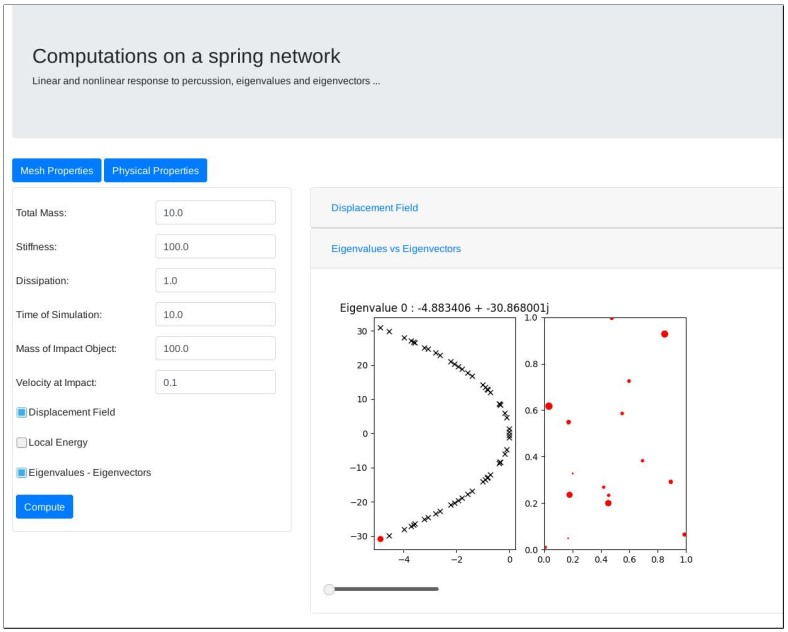
\includegraphics[width=0.85\textwidth]{ClientWebBal.jpg}
    \caption{Client web \texttt{springslattice-web.py} développé dans \parencite[p.197]{balasoiu2020halthesis}.}
    \label{fig:clientwebbal}
\end{figure}




\subsection{Nouveaux travaux sur la percussion}



Les floes de glace $\Omega_k$ et $\Omega_l$ sont modélisés par des systèmes masse-ressort (à grande raideur). Pour l'instant, nous considérons une moélisation simplifiée qui assimile un floe à un système de (trois) masses reliés par des ressorts (de constante de raideur $k$), et par des dispositifs visqueux de constante $\mu$.
Nous désignerons par $n+1$ le nombre total de n\oe{}uds du floe $\Omega_k$, chaque n\oe{}ud ayant pour masse $m$. De facon similaire, on définit les constantes $k'$, $\mu'$, $n'+1$, $m'+1$ pour le floe $\Omega_l$. Les positions des noeds de $\Omega_k$ seront noté $(q_i)_{0\leq i\leq n}$, tandis que ceux de $\Omega_l$ seront notés $(p_i)_{0 \leq i\leq n'-1}$ (voir \cref{fig:contactmanuel}). 

\begin{figure}[!h]
    \centering
    % 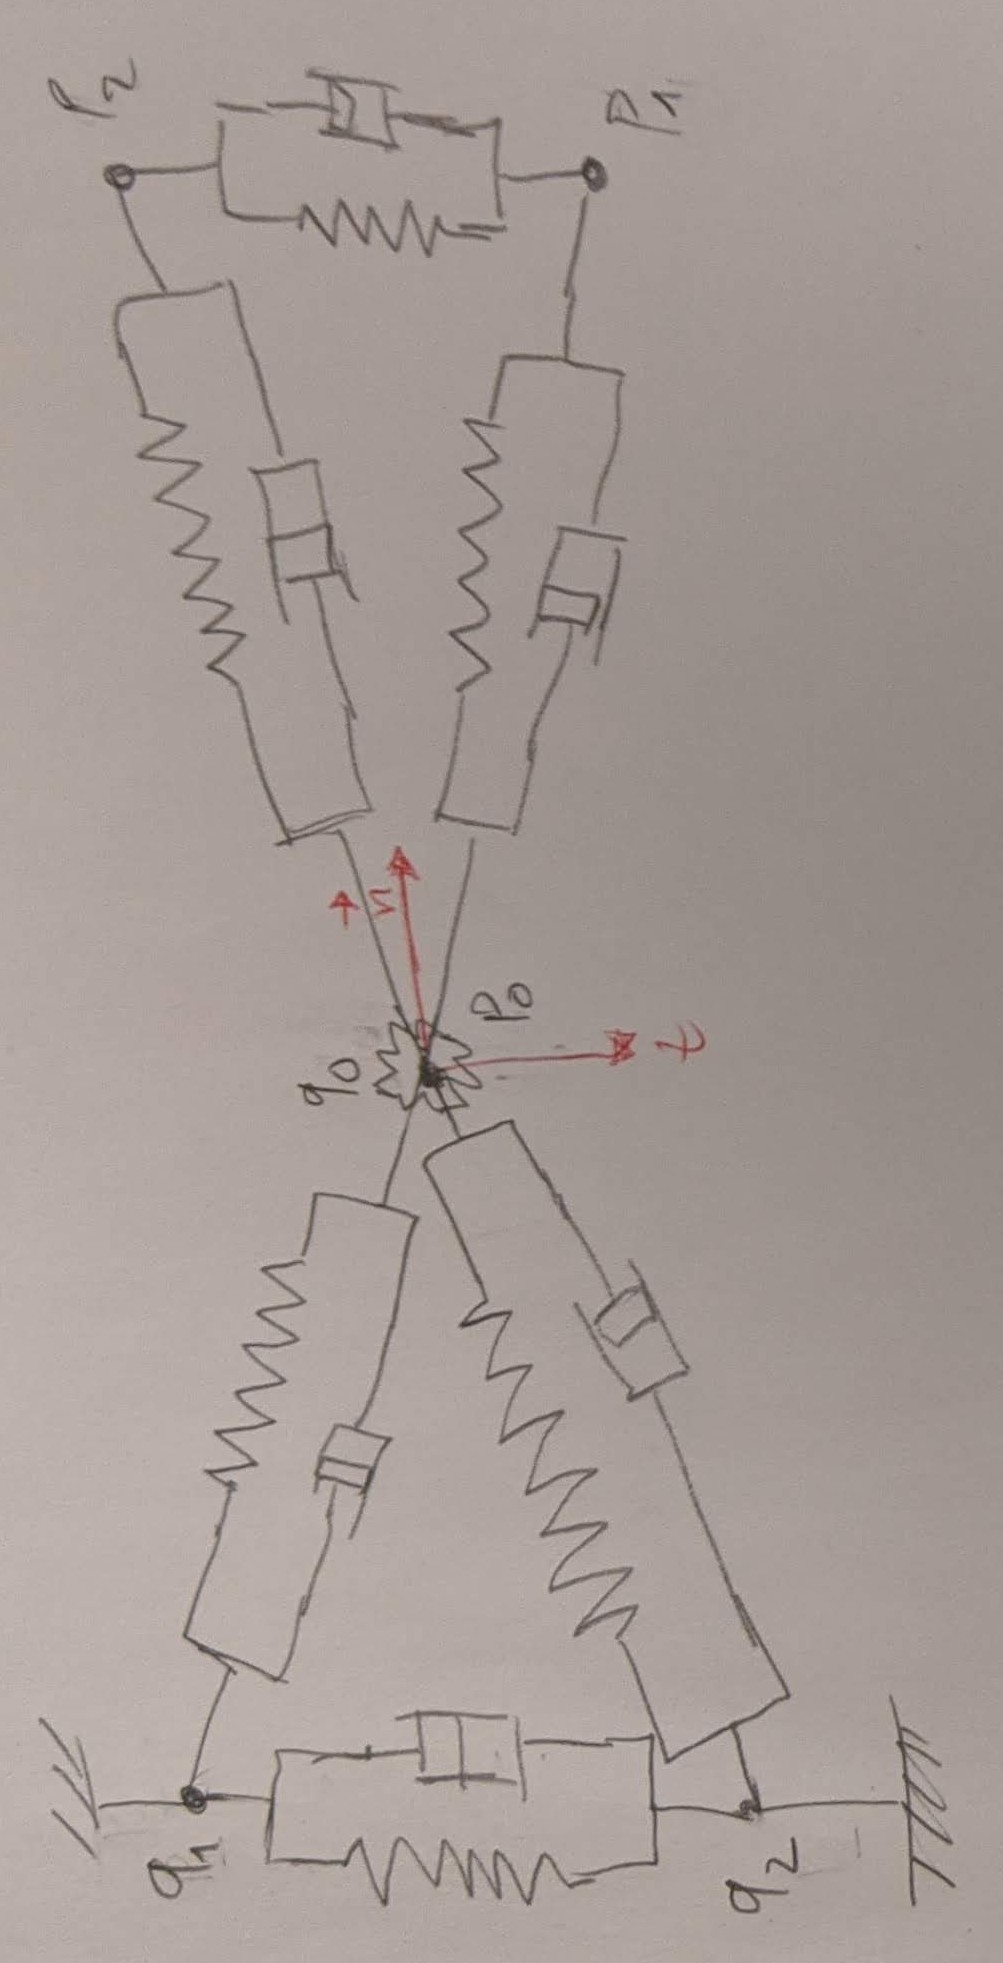
\includegraphics[width=0.3\textwidth, angle=-90]{ContactManuel.jpg}
    \frame{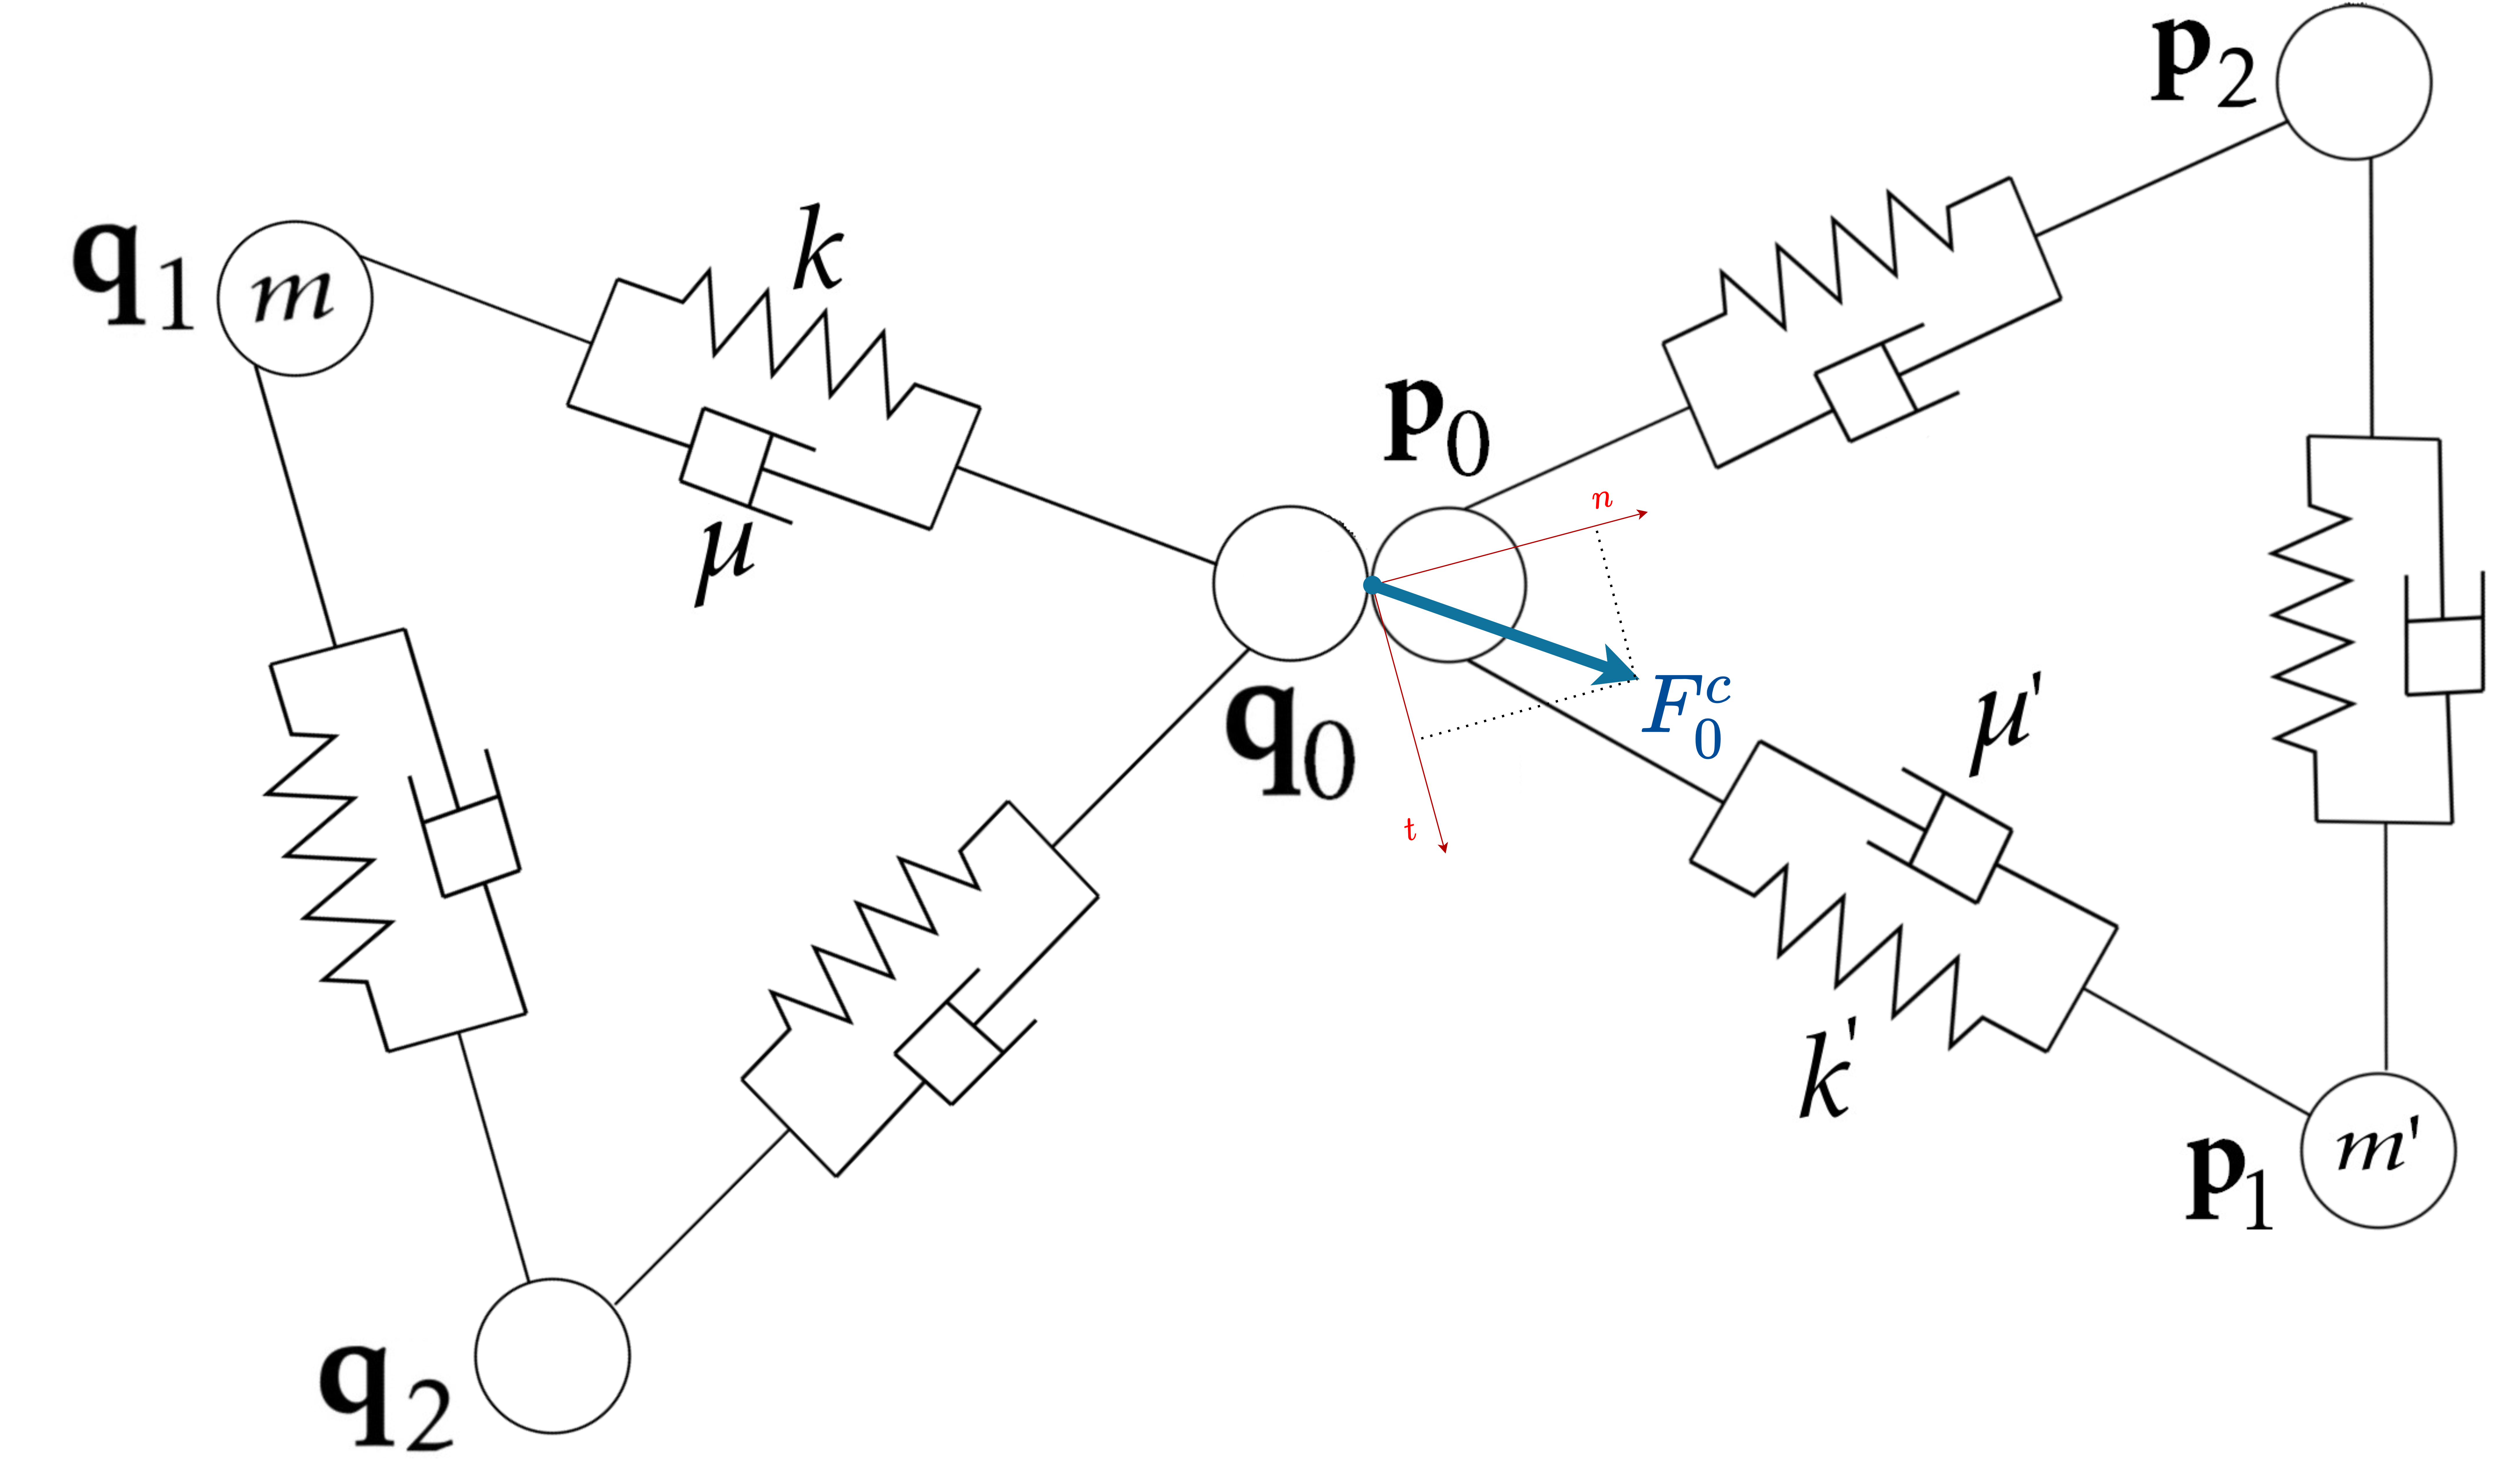
\includegraphics[width=0.65\textwidth]{Percussion2DNew.png}}
    \caption{Contact entre deux floes aux points $\bvec{q}_0$ et $\bvec{p}_0$ respectivement.}
    \label{fig:contactmanuel}
\end{figure}

\noindent On définit la longeur à vide $L_{0j}$ et le vecteur unitaire $\bvec{u}_{0j}$ (orienté de $\bvec{q}_0$ vers $\bvec{q}_j$) entre le n\oe{}ud $\bvec{q}_0$ et le n\oe{}ud $\bvec{q}_j$ et $u_{0j}$. Notons que ces définittions restent valable si nous remplacons le n\oe{}ud $\bvec{q}_0$ par un n\oe{}ud $(\bvec{q}_i)_{0 \leq i \leq n-1}$. On définit aussi la matrice de connectivité $C$:
\begin{align*}
    \forall \, 0 \leq i < j \leq n-1, \quad C_{ij} = C_{ji} = \begin{dcases}
    1 \text{ si } \bvec{q}_i \text{ est voisin de } \bvec{q}_j \,, \\
    0 \text{ sinon }.
\end{dcases}
\end{align*}
\noindent Comme présenté dans les travaux \parencite[p.186]{balasoiu2020halthesis}, le système différentiel qui modélise la percussion s’écrit comme le couplage de deux sous-systèmes. Le premier, dit système intérieur (SI), est à évolution rapide et modélise la propagation des ondes élastiques dans le système masse-ressort. Ici, nous dérivons facilement et réutilisont le SI comme présenté par \citeauthor{balasoiu2020halthesis}. Le second, dit système extérieur (SE), est à évolution lente et modélise la pénétration de l’objet solide dans le système masse-ressorts. Pour dériver le SE sur le floe $\Omega_k$, nous écrivons l'équation de Newton-Euler linéaire\footnote{La rotation du point matériel $q_0$ n'est pas prise en compte ici, d'où l'abscence de l'équation de Newton-Euler angulaire.} au point de contact $q_0$:
\begin{align}  \label{eq:SE}
m \ddot{\bvec{q}}_0 = \bvec{F}_0 + \bvec{F}^c_0 \,,
\end{align}
où 
\begin{align}  \label{eq:F0}
    \bvec{F}_0 = \sum_{j=0}^{n}C_{0j} \left[  \underbrace{k \left( \Vert \bvec{q}_j - \bvec{q}_0 \Vert - L_{0j} \right) \bvec{u}_{0j}}_{\text{Force de rappel}} - \underbrace{\mu \left\langle \bvec{\dot{q}}_j - \bvec{\dot{q}}_0\,, \bvec{u}_{0j}  \right\rangle  \bvec{u}_{0j}}_{\text{Force de dissipation}}  \right] \,,
\end{align}
représente la somme des forces de reaction et de disssipation exercées par le ressort et le dispositif visqueux sur le n\oe{}ud $q_0$ ; et $\bvec{F}^c_0(t)$ la force de contact durant la collison entre les deux particules. En supposnat qu'il existe un repère de contact $\mathcal{R}^c = \{ q_0, \bvec{n}, \bvec{t} \}$ associé au floe $\Omega_k$ (voir \cref{fig:contactmanuel}), on peut écrire, pour $(\lambda, \beta) \in \Rdeux$ :
\begin{align}  \label{eq:F0c}
    \bvec{F}_0^c = \lambda \bvec{n} + \beta \bvec{t} \,.
\end{align}
Le système intérieur (SE) s'obtient facilement en combinant les équations \cref{eq:SE,eq:F0,eq:F0c}. Le système intérieur (SI) s'obtient lui (pour les autres n\oe{}uds du réseau) en y supprimant la force de contact. On obtient au final:
\begin{align} \tag{$E$} \label{eq:e}
\begin{dcases}
    m \ddot{\bvec{q}}_0 = \bvec{F}_0 + \bvec{F}^c_0  \,, &\qquad \text{(SE)} \\
    m \ddot{\bvec{q}}_i = \bvec{F}_i   \,, \quad \quad \quad \forall 1 \leq i \leq n-1 \,. &\qquad \text{(SI)}
\end{dcases}
\end{align}
En ce qui concerne le floe $\Omega_l$, nous procédons de facons similaire et appliqons la 3ème loi de Newton (action-réaction) pour obtenir le système:
\begin{align} \tag{$E'$} \label{eq:eprime}
\begin{dcases}
    m' \ddot{\bvec{p}}_0 = \bvec{F}^{'}_0 - \bvec{F}^c_0  \,, &\qquad \text{(SE)} \\
    m' \ddot{\bvec{p}}_i = \bvec{F}^{'}_i   \,, \quad \quad \quad \forall 1 \leq i \leq n'-1 \,, &\qquad \text{(SI)}
\end{dcases}
\end{align}
où $(\bvec{F}^{'}_i)_{0 \leq i \leq n'}$ sont définis de facon similaire à $\bvec{F}_0$ (voir \cref{eq:F0}):
\begin{align}
    \bvec{F}'_i = \sum_{j=i}^{n'}C_{ij} \left[ k' \left( \Vert \bvec{p}_j - \bvec{p}_i \Vert - L'_{ij} \right) \bvec{u'}_{ij} - \mu' \left\langle \bvec{\dot{p}}_j - \bvec{\dot{p}}_i\,, \bvec{u}'_{ij}  \right\rangle  \bvec{u}'_{ij}  \right] \,.
\end{align}

\noindent Ensuite, on additionne membre à membre les équations des systèmes extérieurs (SE) de \cref{eq:e,eq:eprime} pour éliminer la force de contact. On obtient:
\begin{align}
m \ddot{\bvec{q}}_0 + m' \ddot{\bvec{p}}_0 = \bvec{F}_0 + \bvec{F}^{'}_0 \,.
\end{align}
Remarquons que les positions relatives des n\oe{}uds $\bvec{q}_0$ et $\bvec{p}_0$ restent inchangées durant la collision. A l'instant initial, on note donc $\Delta_0 = \bvec{q}_0(0) - \bvec{p}_0(0)$, et $\bvec{\dot q}_0(0) = \bvec{\dot p}_0(0)$ ; idéalement, nous voudrions que:
\begin{align}
\forall t \in \mathbb{R}^+ \,, \quad \bvec{q}_0(t) - \bvec{p}_0(t) = \Delta_0\,.
\end{align}
Pour satifaire cette condition, nous exhibons autant d'équations nécessaire pour que notre problème de percussion soit bien posé. Elles sont :
\begin{align} \tag{$\mathcal{P}$} \label{eq:problemeP}
\begin{dcases}
    (m+m') \ddot{\bvec{q}}_0  = \bvec{F}_0 + \bvec{F}^{'}_0  \,, &\qquad \text{(SE)} \\
    \ddot{\bvec{p}}_0 = \ddot{\bvec{q}}_0 \,, \quad \dot{\bvec{p}}_0 = \dot{\bvec{q}}_0 \,, \quad \bvec{p}_0 = \bvec{q}_0 - \Delta_0 \,, &\qquad \text{(SE)} \\
    m \ddot{\bvec{q}}_i = \bvec{F}_i   \,, \quad \quad \quad \forall 1 \leq i \leq n-1 \,. &\qquad \text{(SI)} \\
    m' \ddot{\bvec{p}}_i = \bvec{F}^{'}_i   \,, \quad \quad \quad \forall 1 \leq i \leq n'-1 \,, &\qquad \text{(SI)}
\end{dcases}
\end{align}

Quant à la visualisation des résultats, nous avons construit une interface graphique web pour interagir avec le programme. A travers cette interface, nous pouvons modifier tous les parametres du problèmes et lancer des simulations. Un tel exemple se trouve à la figure \cref{fig:clientwebmoi}, et la simulation correspondant peut etre visualisée via \href{ww}{ce lien SEAFILE}. 
\begin{figure}[!h]
    \centering
    \frame{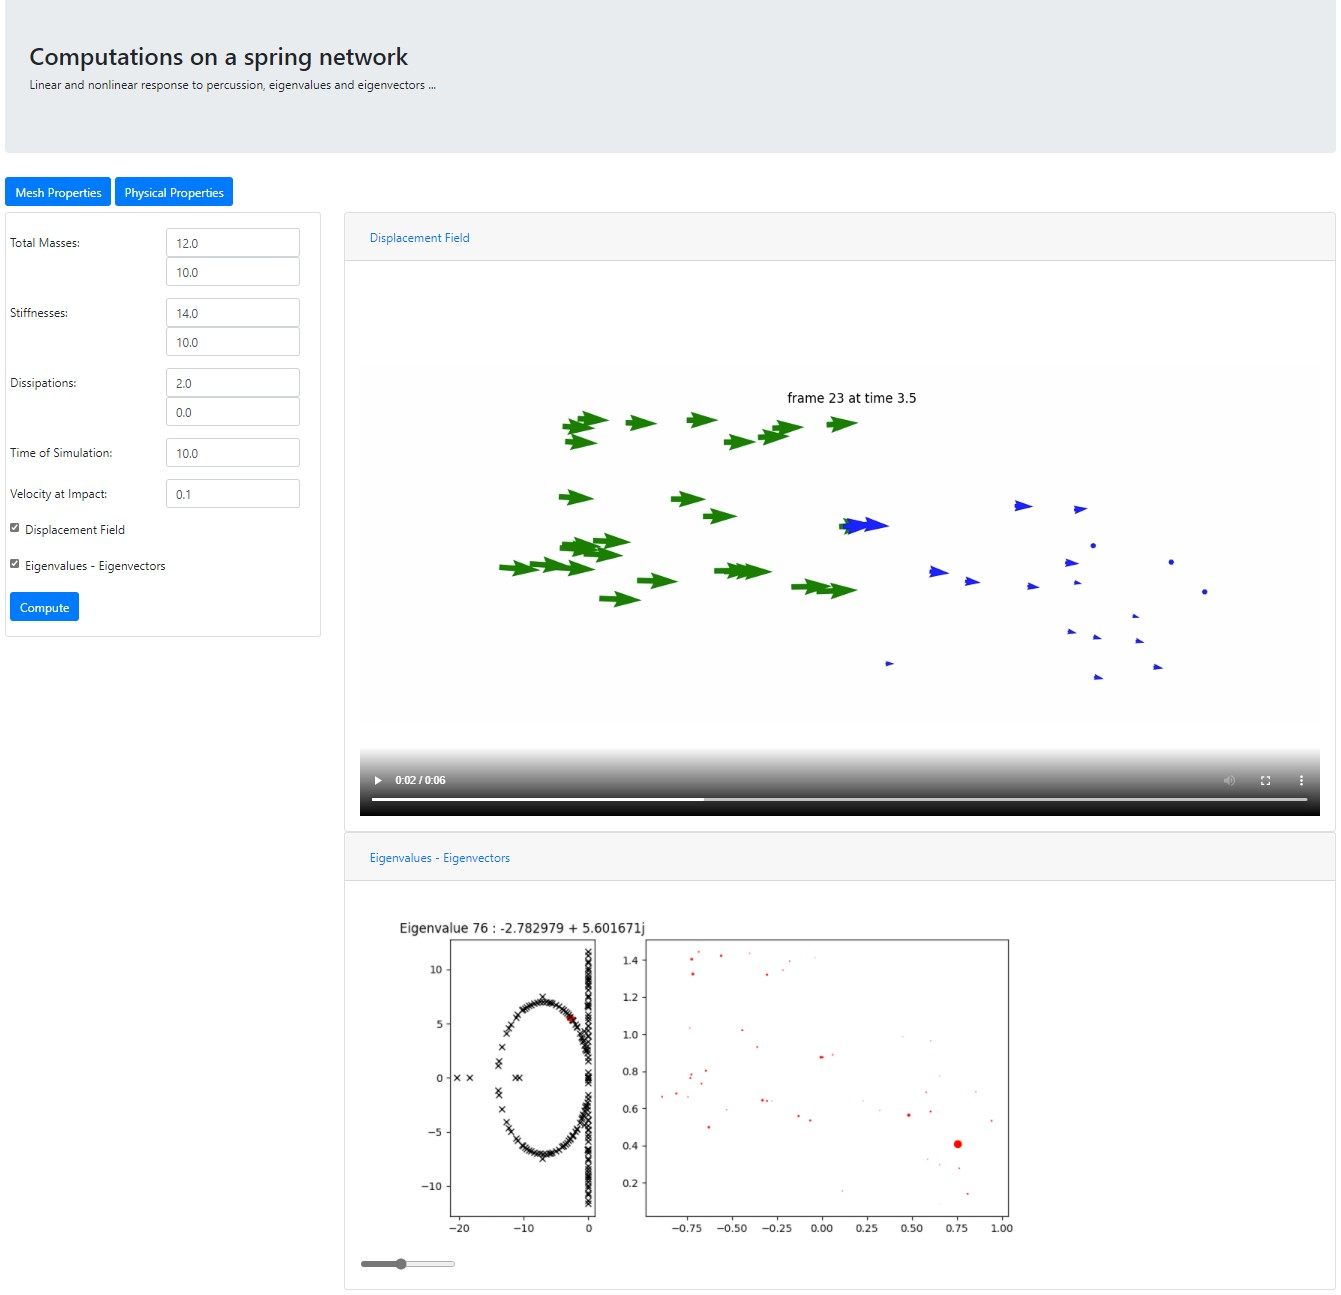
\includegraphics[width=0.85\textwidth]{ClientWebMoi.jpg}}
    \caption{Client web développé durant le stage pour les percussion 2D. Comparativement à la \cref{fig:clientwebbal}, on constate la présence de plus de champ pour préciser les paramètre du second floe entrant en collision.}
    \label{fig:clientwebmoi}
\end{figure}




%3----------------------------------------------------------------------------------------

\section{Code de calcul 2D}


L'algorithme de calcul 2D est largement inspiré des travaux de \citeauthor{balasoiu2020halthesis}. En effet, nous avons ajouté des modules Python à la librarie \texttt{springslattice} qu'il à développé pour traiter les réseaux de ressorts. Ces modules sont:
\begin{enumerate}
    \item \textbf{multimesh}: pour la création d'un réseau de ressort consituté de deux floes de glace en contact, que nous considérerons comme un maillage.
    \item \textbf{multisolver}: pour la création du solveur 2D suivant l'\cref{eq:problemeP} pour simuler les n\oe{}uds d'un objet \texttt{multimesh}. Une fois les caluls fait dans la fonction \texttt{Fhom}, nous les vérifions à l'aide d'un schéma symplectique (voir \cref{AppendixA}).
    \item \textbf{percussion-cli}: pour l'execution des simulations avec des paramètres donnés en ligne de commande (ou ceux insérer par défaut).
    \item \textbf{percussion-web}: pour l'execution des simulations avec des paramètres donnés dans une interface web. Ici, on peut en plus observer les vecteur et les valeurs propres (toutes négatives) du système.
\end{enumerate}

Nous présentons à la \cref{fig:readme2d} le fichier README du dépot \texttt{springslattice} sur \texttt{Framagit} créer par Balasoiu dans ses travaux, et amélioré par nous durant ce stage. Tout comme le dépot principal \href{https://github.com/desmond-rn/ice-floes}{ice-floes} sur \texttt{GitHub}, ce dépot secondaire est privé.
\begin{figure}[!h]
    \centering
    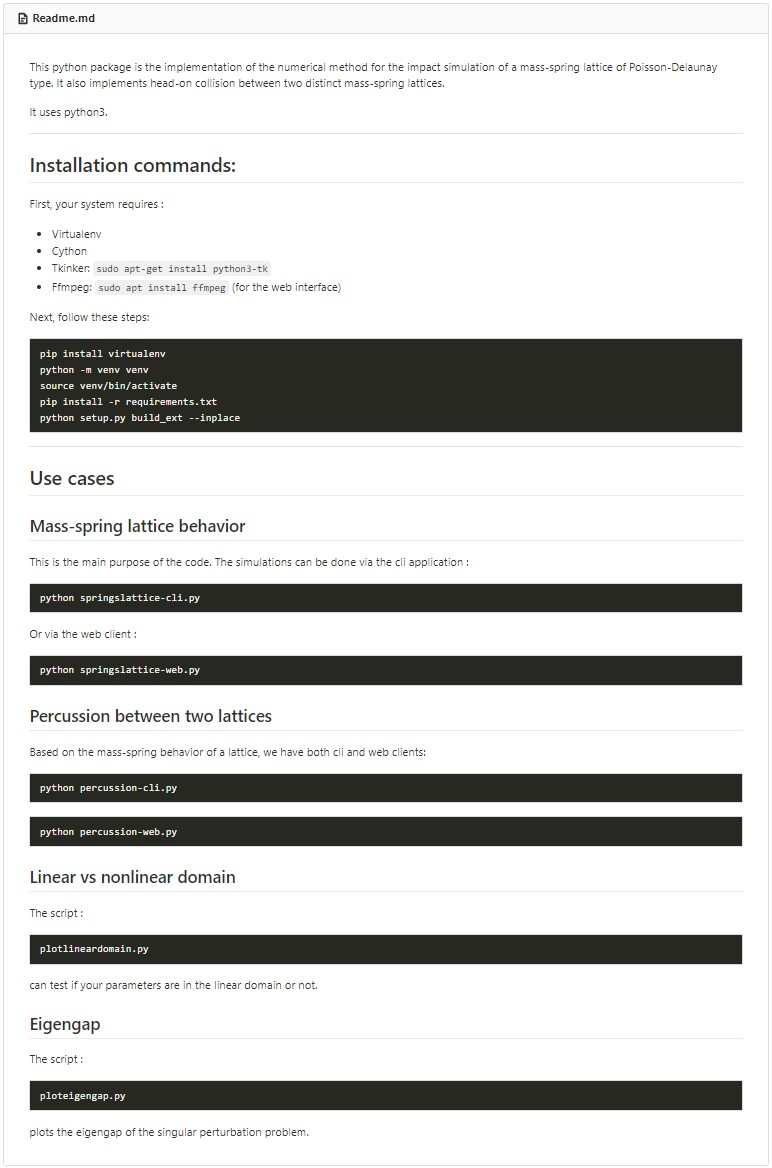
\includegraphics[width=0.85\textwidth]{ReadmeRepoSpringsLattice.jpg}
    \caption{Appercu du dépot secondaire \href{https://framagit.org/RaK/SimuRessorts/-/tree/master}{springslattice} maintenu et amélioré durant le stage.}
    \label{fig:readme2d}
\end{figure}


%4----------------------------------------------------------------------------------------

\section{Résumé des résultats obtenus}

Bien que le modèle de fracture 1D soit facilement adaptable au calculs 2D, nous ne l'avons pas fait fait faute de temps. En particulier, nous avons:
\begin{itemize}
    \item Modélisation du deplacement des n\oe{}uds d'un floe de glace 2D soumis à aucune force sur bord;
    \item Modélisation de le collision (élastique) de deux floe de glace. Vu que le temps de la collision est connu (voir \parencite{rabatel2015thesis}), nous pouvons limiter étendre ces travaux à la collision avec séparation des masses, comme nous l'avons fait en 1D.
    \item Création d'un interface web pour introduire les paramètres et obtenir les résultats d'une simulation. 
\end{itemize}

Les travaux obtenus en 2D sont prometteurs, tout comme ceux obtenu en 1D. Ils ont été obtenu pendant un stage qui a demandé un discipline et une encadrement de taille. Au bout de ce travail, j'ai pu en tirer plusieurs bénéfices.